\documentclass[twocolumn]{article}
\usepackage[english]{babel}
\usepackage[utf8]{inputenc}
\usepackage{amsmath,amssymb,physics,mathtools,blindtext,graphicx}
\usepackage[a4paper,total={7.5in,10in}]{geometry}
\usepackage[labelfont=bf]{caption}

\begin{document}
\begin{large}
\section*{Variational quantum Monte Carlo}
The variational quantum Monte Carlo method (VMC) is a powerful tool to find the ground states of quantum systems. It is especially applicable to many body systems for which analytical approaches, or even direct numerical integration techniques, are impossible. In this report, a despription will be given on the testing of the VMC method on two systems:
\begin{itemize}
    \item[1.] A one dimensional harmonic oscillator.
    \item[2.] A two particle, two dimensional system in which two electrons sit in a harmonic potential and interact with the Coulomb interaction. 
\end{itemize}
The method was used in combination with a golden section search algorithm in order to optimize the variational parameter of the trial functions used.

\subsection*{General procedure}
The energy of the ground state, $E_0$, is a lower bound for the local energy, $E_L$, of any trial function $\psi$:
\begin{equation}
    E_0\leq E_L = \frac{H\psi}{\psi}
\end{equation}
In the VMC method, the positions $x$ are sampled according to the distribution $|\psi|^2$ by means of the Metropolis algorithm. 

The local energy can either be calculated directly or approximated using some finite difference method. 
\begin{itemize}
    \item[1.] Give an interval $[a,b]$ for the variational parameter $\alpha$ where the minimum of $\langle E_L(\alpha)\rangle$ lies. 
    \item[2.] Define two new points on the interval according to the golden section criteria, $c$ and $d$ for which $c<d$, and do Monte Carlo simulations for the trial function with $c$ and $d$ as variational parameters.
    \item[3.] If $\langle E(c)\rangle<\langle E(d)\rangle$, let $b=d$. Otherwise, let $a=c$. Then start again at 2 and continue until a given tolerance or number of iterations is reached. 
\end{itemize}
The Monte Carlo steps were always around 100 000 were the first 10 000 steps were discarded. The trial displacement of the electrons was chosen so that the acceptance ratio was approximately 0.5.


\subsection*{Simple harmonic oscillator}
\begin{figure}[!b]
    % 80000
    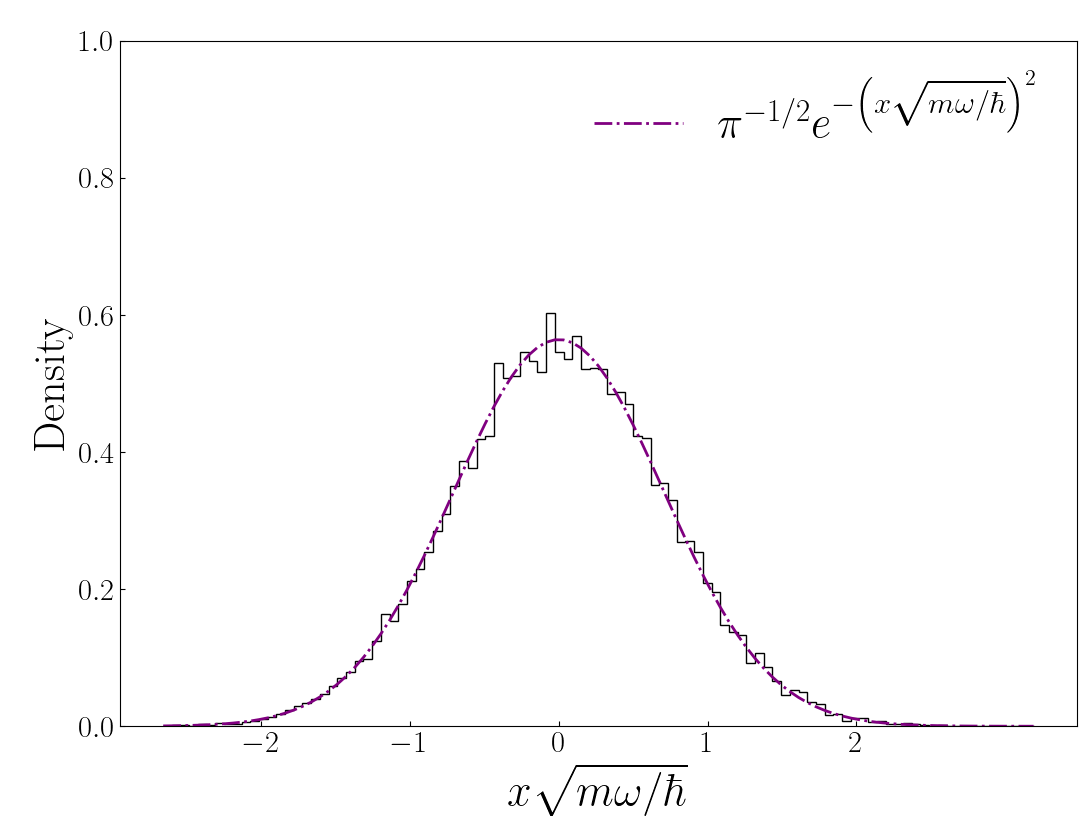
\includegraphics[scale=0.35]{DensityHarOsc.png}
    \caption{The distribution of the positions in a quantum Monte Carlo simulation for the harmonic oscillator. The sum of the histograms is normalized to 1.}
    \label{11apr0918}
\end{figure}
The hamiltonian of the problem is given by
\begin{equation}
    H = -\frac{\hbar^2}{2m}\frac{\text{d}^2}{\text{d}x^2} + \frac{m\omega^2x^2}{2}
\end{equation}
and the trial function is assumed to be a gaussian with a variational parameter $\alpha$:
\begin{equation}
    \psi(x,\alpha) = e^{-\alpha x^2}.
\end{equation}
The local energy of this trial function is then:
\begin{equation}
    E_L(x,\alpha) =\frac{H\psi}{\psi} = \left(\left(1-4\alpha^2\right)x^2m\omega\hbar/2 + \alpha\right)\hbar\omega
\end{equation}
which takes the constant value $E_L=\hbar\omega/2$ for $\alpha = 1/2$. 

The average of the local energy and its variation as function of variational parameters obtained with the combination of VMC and GSS can be seen in figure \ref{10apr1617}. It can be inferred that the minimum is around $\alpha\approx 1/2$. The distribution of the positions is plotted as a histogram in figure \ref{11apr0918}. 
\begin{figure}[t!]
    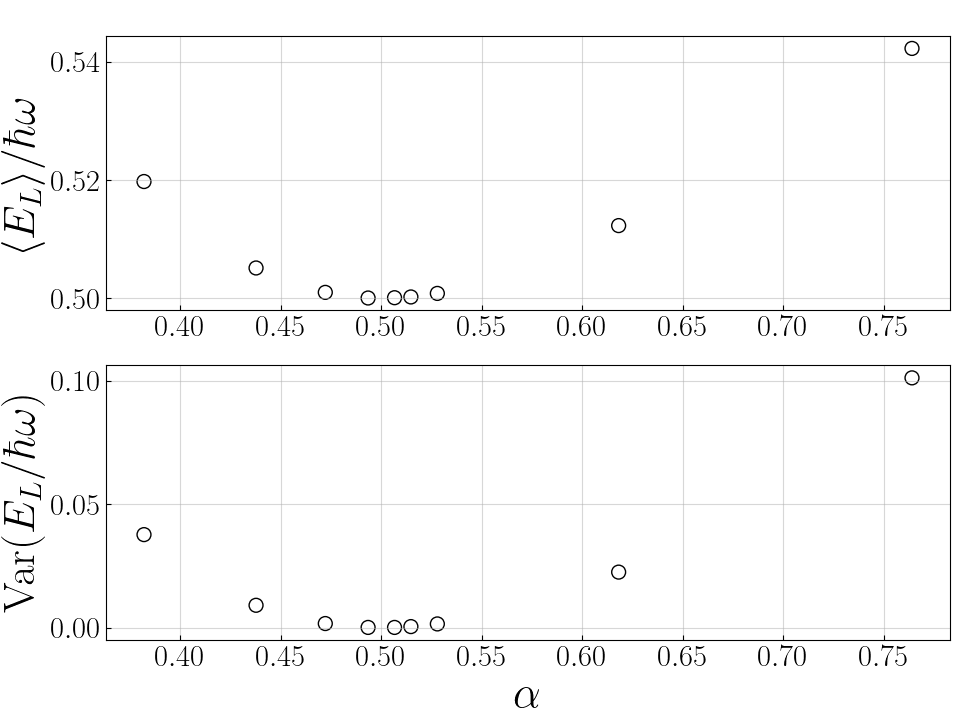
\includegraphics[scale=0.35]{ParamsEnergyHarOsc.png}
    \caption{The average local energy and its variance in a quantum Monte Carlo simulation for the harmonic oscillator, as a function of the variational parameter $\alpha$.}
    \label{10apr1617}
\end{figure}

Another trial function


\subsection*{Harmonic Coulomb potential}
\begin{figure}[!b]
    % 200 000 iters
    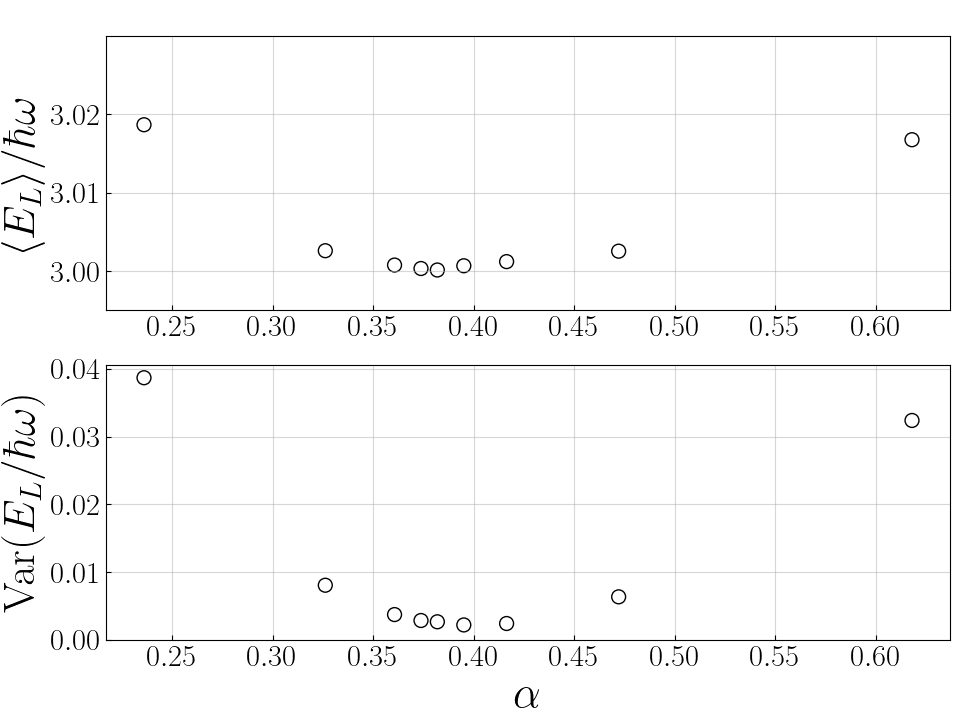
\includegraphics[scale=0.35]{ParamsEnergylambda1.png}
    \caption{The average local energy and its variance as a function of the variational parameter $\alpha$ for interaction parameter $\lambda=1$.}
    \label{11apr0919}
\end{figure}
The hamiltonian for this problem is given by
\begin{equation}
    H = -\frac{1}{2}\big(\boldsymbol{\nabla}_1^2+\boldsymbol{\nabla}_2^2\big) + V_\text{HO} + V_\text{C}
    %\varphi(\mathbf{x}_1,\mathbf{x}_2)
\end{equation}
where reduced units are used in which length is measured in the units of $\sqrt{\hbar/m\omega}$ and energy in the units of $\hbar\omega$. The positions of the electrons are $\mathbf{x}_1 = (x_1,y_1)$ and $\mathbf{x}_2 = (x_2,y_2)$ and the potentials in the hamiltonian are defined by
\begin{equation}
    \begin{split}
        V_\text{HO} = \frac{m\omega^2}{2}\left(r_1^2+r_2^2\right), \quad\quad V_\text{C}  = \frac{\lambda}{r_{12}}.
    \end{split}
\end{equation}
where,
\begin{equation}
    \begin{split}
        & \lambda = \frac{me^2\sqrt{\hbar/m\omega}}{4\pi\epsilon_0\epsilon_r\hbar^2}, \\ 
        &r_1^2 = x_1^2+y_1^2, \quad r_2^2 = x_2^2+y_2^2, \\ 
        &r_{12}^2 = (x_1-x_2)^2+(y_1-y_2)^2. 
    \end{split}
\end{equation}
The parameter $\lambda$ is dimesnionless and is a measure of the strength of the Coulomb interaction. 

The trial function used in the Monte Carlo simulation was:
\begin{equation}
    \psi(x,\alpha) = e^{-(r_1^2+r_2^2)/2}e^{\lambda r_{12}/(1+\alpha r_{12})}
\end{equation}
where $\alpha$ is the variational parameter. The local energy $E_L=H\psi/\psi$ was calculated using a second order finite difference formula for the second derivatives:
\begin{equation}
    \begin{split}
        \frac{\partial^2\psi}{\partial x_1^2}(x_1,y_1,x_2,y_2) &\approx \frac{1}{h^2}\big[\psi(x_1+h,x_2,y_1,y_2) \\ 
        &\hspace{1.3cm}-2\psi(x_1,y_1,x_2,y_2) \\ 
        &\hspace{1.3cm}+\psi(x_1-h,y_1,x_2,y_2) \big]
    \end{split}
\end{equation}
and likewise for the other partial derivaitves. The step size used was $h=10^{-3}$. Testing this trial function for $\lambda=0$ gave $\langle E\rangle = 2$ which is the ground state energy of a two praticle, two dimensional harmonic oscillator. 

The method was then tested for $\lambda\neq 0$. As in the Monte Carlo simulation of the harmonic oscillator, the variational parameter $\alpha$ was varied with a golden section search in order to find the minimum of the local energy for a particular value of $\lambda$. The result for the case $\lambda = 1$ can be seen in figure \ref{11apr0919}. Similar plots were generated for other $\lambda$ and the minimum in local energy was estimated for each case. The results are summarized in figure \ref{11apr2039}.
\begin{figure}[!b]
    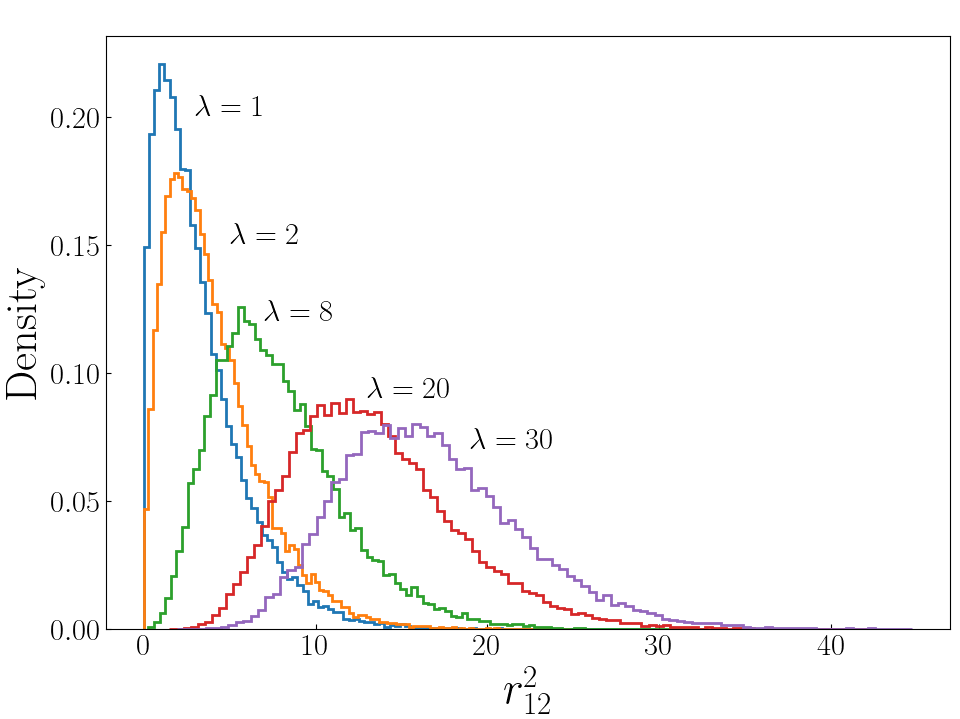
\includegraphics[scale=0.35]{distances.png}
    \caption{The distributions of the squared distances between the two electrons for different coupling constants $\lambda$.}
    \label{11apr2001}
\end{figure}
\begin{figure}[!t]
    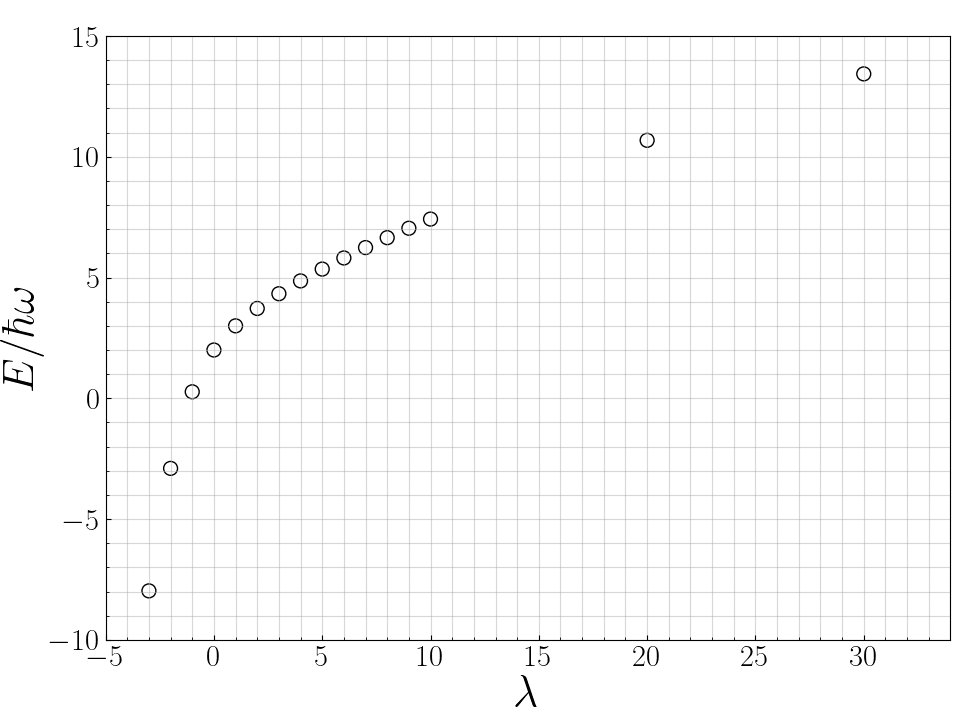
\includegraphics[scale=0.35]{LambdaRelationship.png}
    \caption{The distributions of the squared distances between the two electrons for different coupling constants $\lambda$.}
    \label{11apr2039}
\end{figure}
\begin{figure}[h]
    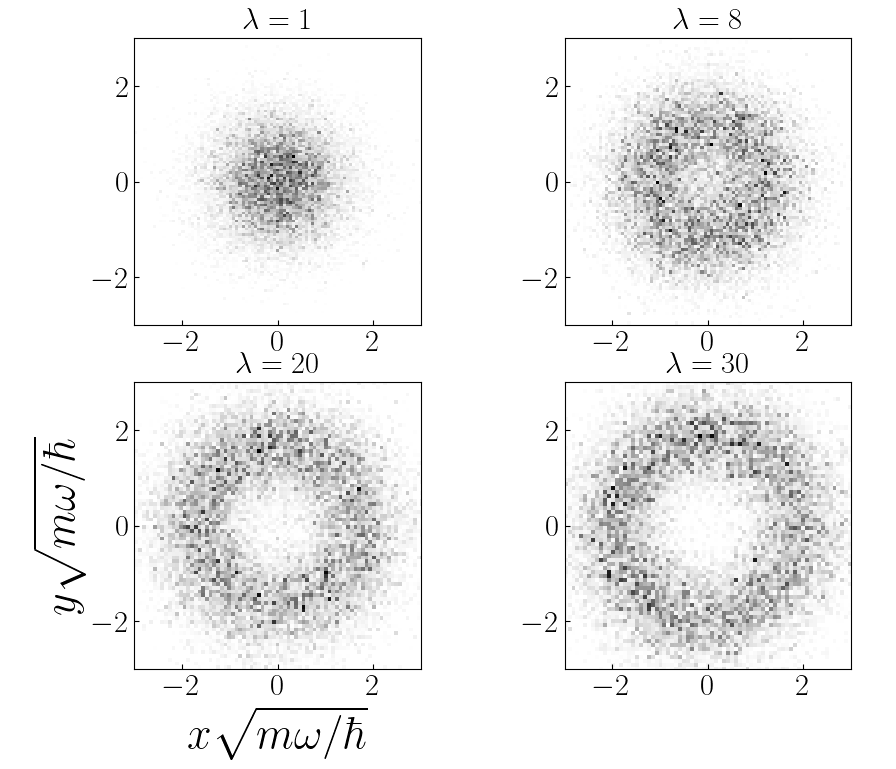
\includegraphics[scale=0.35]{2dhist.png}
    \caption{The distributions of the squared distances between the two electrons for different coupling constants $\lambda$.}
    \label{11apr2120}
\end{figure}



\end{large}
\end{document}
